\chapter{Base knowledge}

Per poter effettuare comunicazioni tramite internet, vi è il bisogno che tutti i dispositivi connessi rispettino determinati meccanismi; questo si rende necessario a causa dell'elevata eterogeneità derivata da hardware e software differenti.
Questi meccanismi, che prendono il nome di \textit{protocolli}, sono strutturati secondo diversi layer (livelli) formando lo stack TCP/IP.  \\
Sebbene l'idea originale prevedesse un modello (ISO/OSI) composto da sette livelli, de facto lo schema attualmente in uso ne prevede solamente quattro. Nonostante ciò, nella terminologia informatica la numerazione dei livelli è rimasta quella precedente.
\\
\begin{table}[htb]
	\centering
	\begin{tabular}{| l | c |}
		\hline
		Livello 7 & Applicativo
		\\
		\hline
		Livello 4 & Trasporto
		\\
		\hline
		Livello 3 & Rete
		\\
		\hline
		Livello 2 & Host-to-network
		\\
		\hline
		
	\end{tabular}
	\caption{Livelli dello stack TCP/IP}
	\label{tab:stack}
\end{table}


\section{Header per il fingerprinting}
Gli header aggiunti ad ogni livello tramite il meccanismo dell'incapsulamento sono formati da vari campi contententi informazioni utili per la comunicazione, e il valore che questi assumono in determinate situazioni è dipendente dal sistema operativo che si sta utilizzando.

Si prenda ad esempio l'header TCP, un protocollo del livello 4 dello stack:\\

\begin{figure}[H]
	\centering
	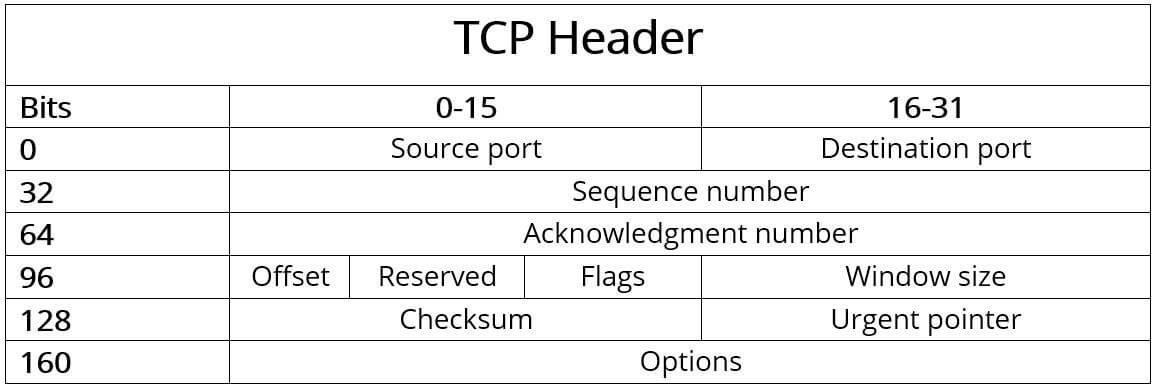
\includegraphics[width=\textwidth]{figures/headerTCP.JPG}
	\caption{Header TCP}
	\label{headerTCP}
	\cite{headerTCP}
\end{figure}

Il campo \textit{option} permette di segnalare al ricevente l'uso di alcune opzioni di comunicazione; il loro supporto e l'effettivo utilizzo, essendo queste facoltative e quindi peculiari di specifici sistemi operativi, rivestono dunque particolare importanza ai fini del fingerprinting.
Esempi analoghi si possono riscontrare nei protocolli ad ogni livello dello stack, e l'unione delle informazioni acquisite dall'analisi degli header consente di poter individuare con una discreta precisione il sistema operativo del dispositivo target.
\\
I test condotti vanno eseguiti successivamente ad alcune operazioni preliminari con lo scopo di effettuare una ricognizione dell'host. Ai fini del fingerprinting attivo è infatti fondamentale effettuare prima un \textit{port scanning}, ovvero un'operazione che consente di individuare le porte aperte e quelle chiuse utile per i test riguardanti il quarto livello dello stack. Nmap effettua di default la scansione di 1000 porte.

\section{Strumenti e sistemi operativi utilizzati}
Per la realizzazione dell'obiettivo sono stati utilizzati due differenti sistemi operativi: Windows 11 e Kali (una distribuzione Linux basata su Debian).
La motivazione della scelta di questi sistemi risiede nel fatto che Kali sia stato progettato per la sicurezza informatica e Windows sia il sistema operativo attualmente più utilizzato.

I tool utilizzati sono stati i seguenti:
\begin{itemize}
	\item \textbf{Nmap} \footnote{\url{https://nmap.org}}: principale strumento per effettuare fingerprinting attivo tramite l'invio di specifici pacchetti (\textit{probe}) costruiti appositamente per massimizzare le differenze ricevute nelle risposte, evidenziando maggiormente le caratteristiche peculiari dei sistemi operativi. Come specificato nella sezione precedente, consente anche di effettuare altre operazioni come ad esempio il \textit{port scanning}.
	\item \textbf{p0f} \footnote{\url{https://www.kali.org/tools/p0f/}}: tool per effettuare fingerprinting passivo. Esso analizza i pacchetti ricevuti da una determinata interfaccia oppure quelli passati tramite un file con estensione pcap. È anche in grado di effettuare fingerprinting a livello 7.
	\item \textbf{Wireshark} \footnote{\url{https://www.wireshark.org/download.html}}: si tratta di uno strumento di sniffing che permette la visualizzazione dei pacchetti inviati e ricevuti dal dispositivo tramite un'interfaccia grafica. Consente inoltre di filtrarli sulla base di determinati campi o protocolli utilizzati.
	\item \textbf{Server Apache} \footnote{\url{https://httpd.apache.org}}: web server che consente di rispondere alle richieste di tipo HTTP/HTTPS. È stato installato sia su Windows 11 che su Kali per poter effettuare il confronto tra le risposte inviate.
	\item \textbf{nginx} \footnote{\url{https://www.nginx.com}}: altro web server, installato per cercare le differenze rispetto al server Apache.
	\item \textbf{Scapy} \footnote{\url{https://scapy.net}}: libreria Python in grado di inviare pacchetti con la possibilità di impostare determinati valori in ogni campo. Molto utile il suo utilizzo per quanto riguarda l'invio di pacchetti "patologici" che stimolano risposte utili ai fini del fingerprinting.
	\item \textbf{nftables} \footnote{\url{https://manpages.debian.org/testing/nftables/nft.8.en.html}}: tool per che permette la manipolazione e il blocco di pacchetti sulla base del loro contenuto negli header.
\end{itemize}


